% Options for packages loaded elsewhere
\PassOptionsToPackage{unicode}{hyperref}
\PassOptionsToPackage{hyphens}{url}
%
\documentclass[
  man,floatsintext]{apa6}
\usepackage{amsmath,amssymb}
\usepackage{lmodern}
\usepackage{iftex}
\ifPDFTeX
  \usepackage[T1]{fontenc}
  \usepackage[utf8]{inputenc}
  \usepackage{textcomp} % provide euro and other symbols
\else % if luatex or xetex
  \usepackage{unicode-math}
  \defaultfontfeatures{Scale=MatchLowercase}
  \defaultfontfeatures[\rmfamily]{Ligatures=TeX,Scale=1}
\fi
% Use upquote if available, for straight quotes in verbatim environments
\IfFileExists{upquote.sty}{\usepackage{upquote}}{}
\IfFileExists{microtype.sty}{% use microtype if available
  \usepackage[]{microtype}
  \UseMicrotypeSet[protrusion]{basicmath} % disable protrusion for tt fonts
}{}
\makeatletter
\@ifundefined{KOMAClassName}{% if non-KOMA class
  \IfFileExists{parskip.sty}{%
    \usepackage{parskip}
  }{% else
    \setlength{\parindent}{0pt}
    \setlength{\parskip}{6pt plus 2pt minus 1pt}}
}{% if KOMA class
  \KOMAoptions{parskip=half}}
\makeatother
\usepackage{xcolor}
\IfFileExists{xurl.sty}{\usepackage{xurl}}{} % add URL line breaks if available
\IfFileExists{bookmark.sty}{\usepackage{bookmark}}{\usepackage{hyperref}}
\hypersetup{
  pdftitle={The effect of stimulus duration on directed forgetting for pictures},
  pdfauthor={Patrick Ihejirika1},
  pdflang={en-EN},
  pdfkeywords={Directed Forgetting, Picture Memory},
  hidelinks,
  pdfcreator={LaTeX via pandoc}}
\urlstyle{same} % disable monospaced font for URLs
\usepackage{graphicx}
\makeatletter
\def\maxwidth{\ifdim\Gin@nat@width>\linewidth\linewidth\else\Gin@nat@width\fi}
\def\maxheight{\ifdim\Gin@nat@height>\textheight\textheight\else\Gin@nat@height\fi}
\makeatother
% Scale images if necessary, so that they will not overflow the page
% margins by default, and it is still possible to overwrite the defaults
% using explicit options in \includegraphics[width, height, ...]{}
\setkeys{Gin}{width=\maxwidth,height=\maxheight,keepaspectratio}
% Set default figure placement to htbp
\makeatletter
\def\fps@figure{htbp}
\makeatother
\setlength{\emergencystretch}{3em} % prevent overfull lines
\providecommand{\tightlist}{%
  \setlength{\itemsep}{0pt}\setlength{\parskip}{0pt}}
\setcounter{secnumdepth}{-\maxdimen} % remove section numbering
% Make \paragraph and \subparagraph free-standing
\ifx\paragraph\undefined\else
  \let\oldparagraph\paragraph
  \renewcommand{\paragraph}[1]{\oldparagraph{#1}\mbox{}}
\fi
\ifx\subparagraph\undefined\else
  \let\oldsubparagraph\subparagraph
  \renewcommand{\subparagraph}[1]{\oldsubparagraph{#1}\mbox{}}
\fi
\newlength{\cslhangindent}
\setlength{\cslhangindent}{1.5em}
\newlength{\csllabelwidth}
\setlength{\csllabelwidth}{3em}
\newlength{\cslentryspacingunit} % times entry-spacing
\setlength{\cslentryspacingunit}{\parskip}
\newenvironment{CSLReferences}[2] % #1 hanging-ident, #2 entry spacing
 {% don't indent paragraphs
  \setlength{\parindent}{0pt}
  % turn on hanging indent if param 1 is 1
  \ifodd #1
  \let\oldpar\par
  \def\par{\hangindent=\cslhangindent\oldpar}
  \fi
  % set entry spacing
  \setlength{\parskip}{#2\cslentryspacingunit}
 }%
 {}
\usepackage{calc}
\newcommand{\CSLBlock}[1]{#1\hfill\break}
\newcommand{\CSLLeftMargin}[1]{\parbox[t]{\csllabelwidth}{#1}}
\newcommand{\CSLRightInline}[1]{\parbox[t]{\linewidth - \csllabelwidth}{#1}\break}
\newcommand{\CSLIndent}[1]{\hspace{\cslhangindent}#1}
\ifLuaTeX
\usepackage[bidi=basic]{babel}
\else
\usepackage[bidi=default]{babel}
\fi
\babelprovide[main,import]{english}
% get rid of language-specific shorthands (see #6817):
\let\LanguageShortHands\languageshorthands
\def\languageshorthands#1{}
% Manuscript styling
\usepackage{upgreek}
\captionsetup{font=singlespacing,justification=justified}

% Table formatting
\usepackage{longtable}
\usepackage{lscape}
% \usepackage[counterclockwise]{rotating}   % Landscape page setup for large tables
\usepackage{multirow}		% Table styling
\usepackage{tabularx}		% Control Column width
\usepackage[flushleft]{threeparttable}	% Allows for three part tables with a specified notes section
\usepackage{threeparttablex}            % Lets threeparttable work with longtable

% Create new environments so endfloat can handle them
% \newenvironment{ltable}
%   {\begin{landscape}\begin{center}\begin{threeparttable}}
%   {\end{threeparttable}\end{center}\end{landscape}}
\newenvironment{lltable}{\begin{landscape}\begin{center}\begin{ThreePartTable}}{\end{ThreePartTable}\end{center}\end{landscape}}

% Enables adjusting longtable caption width to table width
% Solution found at http://golatex.de/longtable-mit-caption-so-breit-wie-die-tabelle-t15767.html
\makeatletter
\newcommand\LastLTentrywidth{1em}
\newlength\longtablewidth
\setlength{\longtablewidth}{1in}
\newcommand{\getlongtablewidth}{\begingroup \ifcsname LT@\roman{LT@tables}\endcsname \global\longtablewidth=0pt \renewcommand{\LT@entry}[2]{\global\advance\longtablewidth by ##2\relax\gdef\LastLTentrywidth{##2}}\@nameuse{LT@\roman{LT@tables}} \fi \endgroup}

% \setlength{\parindent}{0.5in}
% \setlength{\parskip}{0pt plus 0pt minus 0pt}

% Overwrite redefinition of paragraph and subparagraph by the default LaTeX template
% See https://github.com/crsh/papaja/issues/292
\makeatletter
\renewcommand{\paragraph}{\@startsection{paragraph}{4}{\parindent}%
  {0\baselineskip \@plus 0.2ex \@minus 0.2ex}%
  {-1em}%
  {\normalfont\normalsize\bfseries\itshape\typesectitle}}

\renewcommand{\subparagraph}[1]{\@startsection{subparagraph}{5}{1em}%
  {0\baselineskip \@plus 0.2ex \@minus 0.2ex}%
  {-\z@\relax}%
  {\normalfont\normalsize\itshape\hspace{\parindent}{#1}\textit{\addperi}}{\relax}}
\makeatother

% \usepackage{etoolbox}
\makeatletter
\patchcmd{\HyOrg@maketitle}
  {\section{\normalfont\normalsize\abstractname}}
  {\section*{\normalfont\normalsize\abstractname}}
  {}{\typeout{Failed to patch abstract.}}
\patchcmd{\HyOrg@maketitle}
  {\section{\protect\normalfont{\@title}}}
  {\section*{\protect\normalfont{\@title}}}
  {}{\typeout{Failed to patch title.}}
\makeatother
\keywords{Directed Forgetting, Picture Memory\newline\indent Word count: X}
\usepackage{lineno}

\linenumbers
\usepackage{csquotes}
\ifLuaTeX
  \usepackage{selnolig}  % disable illegal ligatures
\fi

\title{The effect of stimulus duration on directed forgetting for pictures}
\author{Patrick Ihejirika\textsuperscript{1}}
\date{}


\shorttitle{Directed Forgetting}

\authornote{

This paper is submitted as partial fulfillment for PSYC 5001.

Correspondence concerning this article should be addressed to Patrick Ihejirika, Postal address. E-mail: \href{mailto:my@email.com}{\nolinkurl{my@email.com}}

}

\affiliation{\vspace{0.5cm}\textsuperscript{1} Brooklyn College of CUNY}

\abstract{
Write your abstract here.
}



\begin{document}
\maketitle

\hypertarget{what-is-memory}{%
\subsection{What is memory?}\label{what-is-memory}}

What is memory and how is it altered? Memory is often inaccurately defined as the ability to encode, store and retrieve information. A more accurate definition separates memory into two separate processes. Process one is characterized by remembering information and is defined as successfully encoding, storing and retrieving information. Process two is characterized by forgetting information. This definition allows for the conceptual introduction of intentionally controlling ones memory by selectively forgetting information details. The process by which information is forgotten can be explored using a directed forgetting procedure.

\hypertarget{what-is-directed-forgetting}{%
\subsection{What is Directed Forgetting?}\label{what-is-directed-forgetting}}

The directed forgetting procedure instructs participants to selectively remember or forget specific events and measures the accuracy with which participants are able to do so (for a review see, MacLeod, 1998). The design of a directed forgetting procedure consists of an encoding phase and a testing phase. The encoding phase presents participants with a series which is then followed by the presentation of instructional cues, directing participants to either remember or forget the previously presented stimulus. After the participants have been presented with all available stimuli, the testing phase begins. This testing phase then presents the same stimuli of the encoding phase against previously unseen stimuli, and tasks participants to accurately identify the stimulus presented in the encoding phase. Significantly lower accuracy in the recognition of forget-cued encoding stimuli is an indication of the presence of a phenomenon known as the directed forgetting effect.

\hypertarget{a-classic-demonstration-of-directed-forgetting}{%
\subsection{A classic demonstration of directed forgetting}\label{a-classic-demonstration-of-directed-forgetting}}

Bjork (1972) provides a description of traditional directed forgetting procedures. Generally, these procedures present participants with a series of items and cues. There are a number of ways to cue various item sets, including intraserial cuing, postinput cuing and pre-input cuing. The most common method of cuing item sets throughout traditional directed forgetting procedures is intraserial cuing. Intra-serial cuing sequentially presents participants with a set of items and directs them to either forget or remember said item using the cue's instruction. Though the item presented during such experiments may vary, traditional directed-forgetting procedures discussed throughout this paper use word stimuli as the presented items.
Traditional directed forgetting procedures also determine the presence and magnitude of a directed forgetting effect using either recognition or recall based testing conditions. Testing conditions which operationalize the directed forgetting effect as the accurate recall of ``Forget-cued'' stimuli do so by having participants recall as many wordage items as possible, without regard to the cue instructions. Previous research employing this recall-based directed forgetting procedure has identified a directed forgetting effect of 10-15\% for F- cued wordage stimuli, compared to the R- cued wordage stimuli (Weiner \& Reed, 1969). Testing conditions which operationalize the directed forgetting effect as the accurate recognition of ``Forget-cued'' stimuli do so by having participants identify as many previously seen wordage items as possible, without regard to the cue instructions.

\hypertarget{what-do-we-empirically-know-about-directed-forgetting}{%
\subsection{What do we empirically know about directed forgetting?}\label{what-do-we-empirically-know-about-directed-forgetting}}

MacLeod (1998) has identified 38 factors with the potential to influence the directed-forgetting effect. This paper will specifically focus on 4 of these 38 factors. These 4 factors include cue presentation time, stimulus presentation time, stimulus detail and stimulus type.

Wetzel (1977) used a directed forgetting procedure to explore the effects of cue duration on the participant recall accuracy of word stimuli. This exploration required the manipulation of both the stimuli presentation duration and the cue presentation duration during the encoding phase, creating two separate experimental conditions. These experimental conditions are known as the long delay condition and the short delay condition. The long-delay condition presents the word stimuli for a duration of 2, 4 or 8 seconds and the cue for a duration of 1 second, while the short-delay condition presents the word stimuli for a duration of 1 second and the cue for a duration of 2, 4 or 8 seconds. The result of this experiment indicates that short delay conditions, specifically conditions with short stimulus duration and long cue duration lead to an increased directed forgetting effect. These results serve as a motivation for the factorial manipulation of stimuli presentation duration within my experiment.

Ahmad, Tan, and Hockley (2019) used a directed forgetting procedure which explored the effects of stimuli details on accuracy of participant recognition of encoding phase stimuli. This was done through the introduction of novel testing conditions and exemplar conditions into the testing phase. Novel conditions present the same stimuli from the encoding phase against previously unseen stimuli, completely different to that of the encoding stimuli. Exemplar conditions present the same stimuli from the encoding phase against previously unseen stimuli similar to that of the encoding stimuli. Both conditions task participants to accurately identify the stimulus presented in the encoding phase. The results of this experiment indicate the existence of a significantly lower directed forgetting effect for novel testing conditions. This indication of significantly higher accuracy in participant recognition for novel testing conditions than exemplar testing conditions serves as a motivation for my experiment.

Traditional directed forgetting experiments employed both recall-based testing procedures and verbage stimuli to determine the existence of a directed forgetting effect amongst participants. Epstein (1972) defines the directed forgetting effect from the more traditional perspective as a significant decrease in participant ability to accurately recall the verbage stimuli presented during the encoding phase from memory. The issue with recall-based directed forgetting procedures, is that they fail to consider inherently more memorable stimuli. Standing (1973) shows that people possess the ability to remember thousands of pictures, along with the object details within said pictures (MacLeod, 1998). Ahmad, Moscovitch, and Hockley (2017) considers this in his experiment through the use of a recognition-based directed forgetting procedure and pictorial stimuli throughout the encoding phase. The results of this experiment indicate that although directed forgetting for pictures and their objects, its effects are extremely small. These results and the memorable ability of images as opposed to word stimuli serves as the motivation for the use of image stimuli throughout my experiment.

\hypertarget{experiment-1}{%
\section{Experiment 1}\label{experiment-1}}

Experiment 1 quite similarly resembles the traditional directed forgetting procedural technique used by Bjork, Laberge, and Legrand (1968) to explore participant recognition of previously seen encoding stimuli when randomly presented with distractors throughout the testing phase. Deviations from Bjork's experimental procedure include (1) the factorial manipulation of stimuli presentation duration by 500 milliseconds, 1 second and 2 seconds (2) the randomized presentation of novel and exemplar distractors throughout the testing phase (3) the use of inherently more memorable stimuli -images- throughout both the encoding and testing phase, instead of word stimuli.

\hypertarget{method}{%
\subsection{Method}\label{method}}

\hypertarget{participants.}{%
\subsubsection{Participants.}\label{participants.}}

All participants in this experiment were from the Amazon Turks online website. In total, 30 subjects participated in Experiment 1. Participants received monetary compensation for participation in this experiment according to current NYC minimum wage rates. All procedures issued by the Brooklyn College Institutional Review Board were followed and consent was received from all subjects throughout each phase of this experiment.

\hypertarget{stimuli-and-apparatus.}{%
\subsubsection{Stimuli and Apparatus.}\label{stimuli-and-apparatus.}}

There were 120 images from a total of 16 categorical scenes presented throughout the encoding phase of this experiment. These sixteen categorical scenes were further classified as being either outdoor scenes or indoor scenes. The eight of sixteen outdoor visual scenes consisted of settings which included bedrooms, churches, classrooms, offices, dining rooms, conference rooms, hair salons \& empty rooms. The eight of sixteen indoor visual scenes consisted of settings such as airports, bridges, beaches, castles, cemeteries, houses, tents and playgrounds. These 120 images were of the same database of 320 total images of 24 different categorical scenes created by Isola, Xiao, Torralba, and Oliva (2011). Brady, Konkle, Alvarez, and Oliva (2008) and Ahmad et al. (2019) made similar use of this image dataset in earlier experiments.

Alongside the initial 120 images presented during the encoding phase, another 120 images were selected as distractors throughout the testing phase. Sixty of these images were of the same visual scene categories as the images presented during the encoding phase. These images were presented as exemplar distractor testing conditions. The other half of the 120 distractor images were of completely new visual scene categories as the images presented throughout the encoding phase. These distractor images were presented as novel distractor testing conditions. This experiment was programmed in JavaScript using Jspsych and was served onto the web using Jatos. The results of this experiment were analyzed using Rcode.

We used R (Version 4.1.0; R Core Team, 2021) and the R-packages \emph{dplyr} (Version 1.0.7; Wickham, François, Henry, \& Müller, 2021), \emph{forcats} (Version 0.5.1; Wickham, 2021a), \emph{ggplot2} (Version 3.3.5; Wickham, 2016), \emph{jsonlite} (Version 1.7.2; Ooms, 2014), \emph{pacman} (Version 0.5.1; Rinker \& Kurkiewicz, 2018), \emph{papaja} (Version 0.1.0.9997; Aust \& Barth, 2020), \emph{purrr} (Version 0.3.4; Henry \& Wickham, 2020), \emph{readr} (Version 2.0.2; Wickham \& Hester, 2021), \emph{stringr} (Version 1.4.0; Wickham, 2019), \emph{tibble} (Version 3.1.6; Müller \& Wickham, 2021), \emph{tidyr} (Version 1.2.0; Wickham, 2021b), \emph{tidyverse} (Version 1.3.1; Wickham et al., 2019), and \emph{tinylabels} (Version 0.2.1; Barth, 2021) for all our analyses. We collected five subjects worth of pilot data. For each subject we computed mean recognition accuracy in each condition of the design. Figure 1 shows mean recognition accuracy in each condition, collapsed across each subject.

\hypertarget{design}{%
\subsubsection{Design}\label{design}}

This experiment consisted of a 2x2x3 completely within-subjects experimental design, with the manipulated variables including the Distractor Test, Cue \& picture encoding time. The distractor testing condition variable possessed two distinct manipulations, being novel testing conditions and exemplar testing conditions. Novel testing conditions display images with previously unseen or unrelated visual scene categories as distractors during the testing phase. Exemplar testing conditions display images with similar visual scene categories as distractors during the testing phase. The picture presentation time variable possessed three distinct manipulations to the duration of images presented during the encoding phase of the experiment. These three manipulations included durations of 500 milliseconds, 1 second and 2 seconds. The cue presentation variable possessed two distinct manipulations. These two manipulations included the ``Remember'' cue and the ``Forget'' cue. The Remember cue instructs participants to remember the upcoming image stimuli, while the ``Forget'' cue instructs participants to selectively forget the upcoming image stimuli.

\hypertarget{procedure.}{%
\subsection{Procedure.}\label{procedure.}}

Participants used the Just Another Tool for Online Studies (JAVOS) site to access the experiment. As stated earlier, there are two major phases of the experiment. These phases are the encoding phase and the testing phase. Prior to the encoding phase however, participants were presented with a consent form. Upon completion of the consent form, they were presented with encoding phase instructions.

During the encoding phase, participants are presented with the cue instructions followed by the images. The cues instruct participants to either selectively remember or selectively forget the upcoming image stimuli at random. There are a total of 120 cue instructions, which are presented for a duration of (XXXX) seconds. The image stimuli presented during the encoding phase are composed of the 120 images from a total of 16 categorical scenes subsetted from the larger database of 320 images with a total of 24 categorical scenes. These 120 images are presented at random at durations of either 500 milliseconds, 1 second or 2 seconds. The presentation times of the images will also be displayed at random. Seeing as how the presentation of a single cue instruction followed by a single image consists of a single trial, and there are 120 cue instructions and 120 images to be presented, then there will be 120 trials throughout the encoding phase of this experiment.

Upon completion of the encoding phase, participants were then taken to the testing phase. Similarly to the encoding phase, during the beginning of the testing phase participants were given instructions of completing the testing phase. During the testing phase, participants are given a series of trials where they are shown either an exemplar distractor image or a novel distractor image alongside an image previously seen during the encoding phase and are tasked with selecting the encoding image. There are 60 novel distractor images and 60 exemplar distractor images, each of which were presented at random throughout the testing procedure.

\hypertarget{results}{%
\subsection{Results}\label{results}}

\begin{figure}
\centering
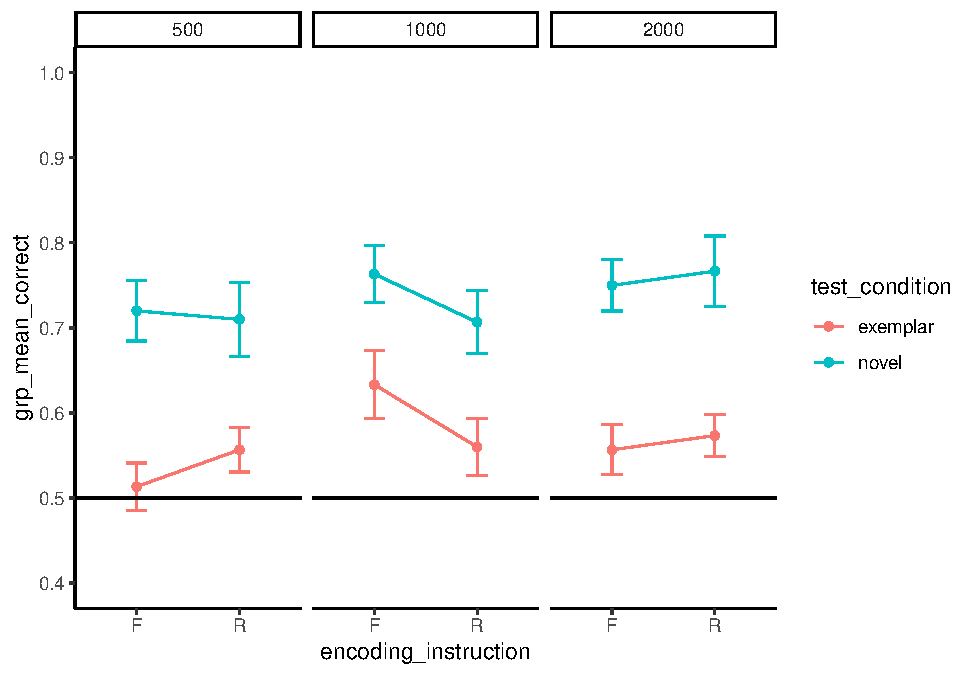
\includegraphics{honorsThesis_files/figure-latex/e1fig-1.pdf}
\caption{\label{fig:e1fig}This is the figure caption.}
\end{figure}

The proportion of accurately recognized encoding stimuli was collected for each of the subjects who participated in the pilot study. The recorded proportions were then averaged according to the conditions present in this 2x2x3 within subjects experimental design. Mean proportion correct for each subject was then submitted to a 2: Cue instruction conditions (R vs F), by 2: Test conditions (Novel vs Exemplar), by 3: Stimulus duration conditions (500ms vs 1000ms vs 2000ms), repeated measures analysis of variance.

The main effect of encoding time was, \(F(2, 58) = 2.78\), \(\mathit{MSE} = 0.02\), \(p = .070\), \(\hat{\eta}^2_G = .010\). Proportion correct was 0.62 (0.02), 0.67 (0.02), and 0.66 (0.02) for the 500ms, 1000ms, and 2000ms intervals, respectively.

The main effect of test lure was significant, \(F(1, 29) = 67.82\), \(\mathit{MSE} = 0.04\), \(p < .001\), \(\hat{\eta}^2_G = .177\). Proportion correct was higher for novel lures (0.74, SEM = 0.02), compared to exemplar lures (0.57, SEM = 0.01).

The main effect of encoding instruction was, \(F(1, 29) = 0.59\), \(\mathit{MSE} = 0.02\), \(p = .448\), \(\hat{\eta}^2_G = .001\). Proportion correct was similar for forget cued (0.66, SEM = 0.02) and remember cued (0.65, SEM = 0.02) items

The interaction between encoding instruction and encoding time was significant, \(F(2, 58) = 4.40\), \(\mathit{MSE} = 0.02\), \(p = .017\), \(\hat{\eta}^2_G = .011\). To further interpret this interaction, paired sample t-tests were used to assess the directed forgetting effect at each encoding time duration. The directed forgetting effect is taken as the difference between proportion correct for remember minus forget items. At 500 ms, the directed forgetting effect was not detected, \(M = 0.02\), 95\% CI \([-0.03, 0.06]\), \(t(29) = 0.75\), \(p = .458\). At 1000ms, the directed forgetting effect was reversed, \(M = -0.06\), 95\% CI \([-0.11, -0.02]\), \(t(29) = -2.67\), \(p = .012\). And, at 2000 ms, the directed forgetting effect was again not detected, \(M = 0.02\), 95\% CI \([-0.03, 0.06]\), \(t(29) = 0.75\), \(p = .458\). The remaining interactions were not significant.

\hypertarget{discussion}{%
\subsection{Discussion}\label{discussion}}

Statistical analysis of pilot data indicates the presence of a significant directed forgetting effect for Testing conditions, as participant accuracy in novel conditions is significantly greater compared to participant accuracy in exemplar conditions. A potential explanation of this difference in accuracy lies within the visual scene details information processed by participants during novel conditions versus exemplar conditions. Since novel testing conditions present distractor images from completely different categories than those shown in the encoding phase, less specific or gist information of the visual scenes details suffices. With less visual scene details required for visual scene processing in novel conditions relative to exemplar conditions, more gist information can be processed and stored in long term memory (Ahmad et al., 2017) with greater efficiency. This efficient storage of gist information in long term memory may explain the difference in performance across testing conditions.

A directed forgetting effect fails to exist for both cue instruction and stimulus presentation duration conditions however, as there are no such significant differences in performance between R or F cues and 500ms, 1000ms or 2000ms.

\newpage

\hypertarget{references}{%
\section{References}\label{references}}

\begingroup
\setlength{\parindent}{-0.5in}
\setlength{\leftskip}{0.5in}

\hypertarget{refs}{}
\begin{CSLReferences}{1}{0}
\leavevmode\vadjust pre{\hypertarget{ref-ahmadEffectsVaryingPresentation2017}{}}%
Ahmad, F. N., Moscovitch, M., \& Hockley, W. E. (2017). Effects of varying presentation time on long-term recognition memory for scenes: {Verbatim} and gist representations. \emph{Memory \& Cognition}, \emph{45}(3), 390--403. \url{https://doi.org/gmgg4q}

\leavevmode\vadjust pre{\hypertarget{ref-ahmadDirectedForgettingCategorised2019}{}}%
Ahmad, F. N., Tan, P., \& Hockley, W. E. (2019). Directed forgetting for categorised pictures: Recognition memory for perceptual details versus gist. \emph{Memory}, \emph{27}(7), 894--903. \url{https://doi.org/gmgg3g}

\leavevmode\vadjust pre{\hypertarget{ref-R-papaja}{}}%
Aust, F., \& Barth, M. (2020). \emph{{papaja}: {Prepare} reproducible {APA} journal articles with {R Markdown}}. Retrieved from \url{https://github.com/crsh/papaja}

\leavevmode\vadjust pre{\hypertarget{ref-R-tinylabels}{}}%
Barth, M. (2021). \emph{{tinylabels}: Lightweight variable labels}. Retrieved from \url{https://github.com/mariusbarth/tinylabels}

\leavevmode\vadjust pre{\hypertarget{ref-bjorkTheoreticalImplicationsDirected1972}{}}%
Bjork, R. A. (1972). Theoretical implications of directed forgetting. In A. W. Melton \& E. Martin (Eds.), \emph{Coding processes in human memory} (pp. 217--235). {Washington, DC}: {Winston}.

\leavevmode\vadjust pre{\hypertarget{ref-bjorkModificationShorttermMemory1968}{}}%
Bjork, R. A., Laberge, D., \& Legrand, R. (1968). The modification of short-term memory through instructions to forget. \emph{Psychonomic Science}, \emph{10}(2), 55--56. \url{https://doi.org/gmt488}

\leavevmode\vadjust pre{\hypertarget{ref-bradyVisualLongtermMemory2008}{}}%
Brady, T. F., Konkle, T., Alvarez, G. A., \& Oliva, A. (2008). Visual long-term memory has a massive storage capacity for object details. \emph{Proceedings of the National Academy of Sciences}, \emph{105}(38), 14325--14329. \url{https://doi.org/c268jz}

\leavevmode\vadjust pre{\hypertarget{ref-EpsteinW1972}{}}%
Epstein, D. W. W., William. Massaro. (1972). Selective search in directed forgetting. \emph{Journal of Experimental Psychology}, \emph{94}(1), 18--24. \url{https://doi.org/10.1037/h0032791}

\leavevmode\vadjust pre{\hypertarget{ref-R-purrr}{}}%
Henry, L., \& Wickham, H. (2020). \emph{Purrr: Functional programming tools}. Retrieved from \url{https://CRAN.R-project.org/package=purrr}

\leavevmode\vadjust pre{\hypertarget{ref-Isola2011}{}}%
Isola, P., Xiao, J., Torralba, A., \& Oliva, A. (2011). What makes an image memorable? \emph{IEEE conference on computer vision and pattern recognition (CVPR)}, 145--152.

\leavevmode\vadjust pre{\hypertarget{ref-macleodDirectedForgetting1998}{}}%
MacLeod, C. M. (1998). Directed forgetting. In J. M. Golding \& C. M. MacLeod (Eds.), \emph{Intentional forgetting: {Interdisciplinary} approaches} (pp. 1--57). {Mahwah, NJ}: {Lawrence Erlbaum Associates}.

\leavevmode\vadjust pre{\hypertarget{ref-R-tibble}{}}%
Müller, K., \& Wickham, H. (2021). \emph{Tibble: Simple data frames}. Retrieved from \url{https://CRAN.R-project.org/package=tibble}

\leavevmode\vadjust pre{\hypertarget{ref-R-jsonlite}{}}%
Ooms, J. (2014). The jsonlite package: A practical and consistent mapping between JSON data and r objects. \emph{arXiv:1403.2805 {[}Stat.CO{]}}. Retrieved from \url{https://arxiv.org/abs/1403.2805}

\leavevmode\vadjust pre{\hypertarget{ref-R-base}{}}%
R Core Team. (2021). \emph{R: A language and environment for statistical computing}. Vienna, Austria: R Foundation for Statistical Computing. Retrieved from \url{https://www.R-project.org/}

\leavevmode\vadjust pre{\hypertarget{ref-R-pacman}{}}%
Rinker, T. W., \& Kurkiewicz, D. (2018). \emph{{pacman}: {P}ackage management for {R}}. Buffalo, New York. Retrieved from \url{http://github.com/trinker/pacman}

\leavevmode\vadjust pre{\hypertarget{ref-standingLearning10000Pictures1973}{}}%
Standing, L. (1973). Learning 10000 pictures. \emph{The Quarterly Journal of Experimental Psychology}, \emph{25}(2), 207--222. \url{https://doi.org/fnjhs5}

\leavevmode\vadjust pre{\hypertarget{ref-WetzelC1977}{}}%
Wetzel, R. E., Douglas C. Hunt. (1977). Cue delay and the role of rehearsal in directed forgetting. \emph{Journal of Experimental Psychology: Human Learning and Memory}, \emph{3}(2), 233--245. \url{https://doi.org/10.1037/0278-7393.3.2.233}

\leavevmode\vadjust pre{\hypertarget{ref-R-ggplot2}{}}%
Wickham, H. (2016). \emph{ggplot2: Elegant graphics for data analysis}. Springer-Verlag New York. Retrieved from \url{https://ggplot2.tidyverse.org}

\leavevmode\vadjust pre{\hypertarget{ref-R-stringr}{}}%
Wickham, H. (2019). \emph{Stringr: Simple, consistent wrappers for common string operations}. Retrieved from \url{https://CRAN.R-project.org/package=stringr}

\leavevmode\vadjust pre{\hypertarget{ref-R-forcats}{}}%
Wickham, H. (2021a). \emph{Forcats: Tools for working with categorical variables (factors)}. Retrieved from \url{https://CRAN.R-project.org/package=forcats}

\leavevmode\vadjust pre{\hypertarget{ref-R-tidyr}{}}%
Wickham, H. (2021b). \emph{Tidyr: Tidy messy data}. Retrieved from \url{https://CRAN.R-project.org/package=tidyr}

\leavevmode\vadjust pre{\hypertarget{ref-R-tidyverse}{}}%
Wickham, H., Averick, M., Bryan, J., Chang, W., McGowan, L. D., François, R., \ldots{} Yutani, H. (2019). Welcome to the {tidyverse}. \emph{Journal of Open Source Software}, \emph{4}(43), 1686. \url{https://doi.org/10.21105/joss.01686}

\leavevmode\vadjust pre{\hypertarget{ref-R-dplyr}{}}%
Wickham, H., François, R., Henry, L., \& Müller, K. (2021). \emph{Dplyr: A grammar of data manipulation}. Retrieved from \url{https://CRAN.R-project.org/package=dplyr}

\leavevmode\vadjust pre{\hypertarget{ref-R-readr}{}}%
Wickham, H., \& Hester, J. (2021). \emph{Readr: Read rectangular text data}. Retrieved from \url{https://CRAN.R-project.org/package=readr}

\end{CSLReferences}

\endgroup


\end{document}
